\documentclass[../eva1_scion.tex]{subfiles}
\begin{document}
    
\section{Results} \label{sec:results}
    In this section, we present the results of our literature research and describe the current state of the proposed SCION architecture. We examine the anatomy of \textit{Isolation Domains} (ISD) and elaborate how the SCION control and data plane work, as well as examining trust management in SCION and deployment status.

    \subsection{Isolation Domains} \label{ssec:isd}
    SCION is designed for easy adoption by current BGP ASes; therefore it adopts and alters some ideas from BGP like the idea of an Autonomous System (AS) which, like in BGP, represents the smallest organizational unit. However, SCION introduces an additional organizational unit called the Isolation Domain (ISD). The structure of an individual ISD is illustrated in \ref{fig:isd}a. 

            An ISD shares a common set of operational rules and a set of trust roots. It is expected that ISDs will grow along social, political and economical borders and structures \cite{scion_2011}. Landing the technical implementation of an ISD a common legal and contractual framework and social context, from which enforceability and a (for humans) meaningful sense of trust can be derived. To emulate these real-world structures, SCION supports recursive ISDs  which inherit trust roots and rules from their parent ISDs \cite{scion_2011}. As an example, one might imagine the tier-1 providers in a country forming the ISD core of a country level ISD, which is a member of an ISD representing a larger geopolitical entity like the EU. Inside a country, there might be a group of ASes which have stronger requirements regarding security and trust than the rest of the ISD; thus they may form a subISD inside the subISD of the country. One such example may be military and its associated organizations.

    \begin{figure}[ht]
        \centering
        \includegraphics[width=0.8\linewidth]{scion_topology.png}
        \caption{A hypothetical topology of ISDs each with their ISD core and member ASes. Image taken from \cite{scion_2015}}%
        \label{fig:isd_topology}
    \end{figure}

    \subsubsection{IDS Structure} \label{sssec:isd_structure}
    As shown in illustration \ref{fig:isd}a the main structure of an IDS is an undirected graph formed by a set of core ASes in the ISD core, client ASes, and bidirectional links between individual ASes. ASes may be connected by multiple redundant links. Although a link always carries bidirectional traffic, there is an implied top down hierarchy of providers and consumers between the tiers in the graph. As in BGP a pair of ASes may enter a peering agreement, which is illustrated is a dashed line. Links are also called path segments.

    An ISD core is composed of multiple core ASes which form a fully connected clique and a logical unit. The ISD core hosts numerous function such as the ISDs certificate authority, core beacon-, certificate-, path-, and address-servers. The ISD core also maintains the \textit{Trust Root Configuration} (TRC). Furthermore, the ISD core  provides links to other ISDs.  Requirement to becoming a core AS is usually sufficient size or importance to offer direct connections to other core ASes in other ISDs, as well as the ability to replicate the other core services listed above \cite{scion_2011}.

    An unassociated AS can join an existing ISD by purchasing connectivity from an ISD which is already member of a given ISD. This requires the joining AS to accept the TRC and operational rules of the ISD it wishes to join. Each AS can be a member of multiple ISDs.

    \subsubsection{AS and ISD Components} \label{sssec:as_componants}

    In the following we will explore the components which are required to run an SCION AS and by extension an ISD since each AS usually replicates all or most core services for caching purposes.

    SCION ASes look similar too their BGP cousins, so fare as that they have internal and border routers and a set of routes through the AS. These ensure connectivity inside the AS and to neighbouring ASes. Border routers must be SCION capable and must adhere to the common rules agreed upon inside the ISD. However, each AS is free to choose its internal structure, such as the intra domain routing protocol and addressing schema. Initially SCION was designed to employ \textit{Accountable Internet Protocol} (AIP) \cite{scion_2011, aip_2008} in all ASes, however this requirement has been relaxed later in favour of interoperability and ease of adoption \cite{scion_2015}. Because of the way SCION forwards packets, there is also no need for a uniform addressing schema between ASes (see \ref{ssec:data_plane}).

    In addition, each AS needs at least a beacon server, a certificate server and a path server. Beacon servers are responsible for path discovery and are required for beaconing process described in section \ref{sssec:beaconing}. Path server are responsible for caching and dissemination of path information. They are involved in path resolution and assembly discussed in section \ref{sssec:path_assembly}. As SCION makes extensive use of certificates to validate paths and entities \cite{scion_2011}, certificate servers are deployed to cache and provide certificates in an AS.

    A core AS differs from other ASes in several important aspects. Most importantly, core ASes have border routers which are connected to cores ASes in neighbouring ISD. Further, the beacon servers in the core ASes also take part in inter ISD beaconing (see section \ref{sssec:beaconing}), thus their path servers also hold path information on how to reach neighbouring ISDs. As mentioned above, the ISD core is responsible for maintaining the trust root configuration (TRC).

    The \textit{Trust Root Configuration} (TRC) is the policy which governs the operations of an ISD. The TRC lists the trust roots used in an ISD and thus is the central anchor of trust in an ISD. It is negotiated between the members of the ISD core, and all ASes wishing to join an ISD, need to accept the TRC. Neighbouring ISDs acknowledge an ISDs TRC by signing it. This makes ASes communicating across ISD borders able to trust signatures originating from a neighbouring ISD. Each TRC also holds a number of policies on how the TRC is used and modified. Modifications to the TRC are only possible of multiple core ASes signed the updated TRC, which prevents a rouge core AS from corrupting the TRC. The number of required signatures for different kinds of changes is governed by the policies encoded in the TRC.

    \subsection{Control Plane} \label{ssec:control_plane}
    Until now, we looked at the static components which constitute an ISD; however, the real-world internet is not a static thing, so an ISD isn't either. To better manage complexity, SCION is divided into a control plane and a data plane. The control plane is concerned with discovering and maintaining paths, while the data plane uses these paths in the processes of path assembly and packet forwarding. This division not only isolates complexity, but also isolates failures and attacks. As long as there are paths available to forward packets on, the data plane can operate without disruption, even if parts of the control plane are disrupted.

    \subsubsection{Path Discovery by Beaconing}\label{sssec:beaconing}
    As mentioned above, SCION has taken inspiration from BGP, the path-discovery mechanism is another place where this is evident. Like in BGP, SCION uses a beaconing process to discover all available paths between ASes. However, unlike in BGP in SCION beacons are not broadcast by every AS to every connected AS, also each AS has control over the paths by which it would like to by reachable. In BGP, an AS has no control over which routes its neighbouring ASes propagate. Beacons in SCION are called \textit{Path-Segment Construction Beacon}s (PCB) and are  sent from beacon servers in the ISD core to travel down the ISD graph as a policy constrained multipath flood. \cite{scion_2011}.

    Initially, the path server in a core ISD issues a PCB containing only the exit interface it originates from and the current version number of the TRC. A path server in a neighbouring AS receiving an incoming PCB will first check the validity of the beacon's signature and then proceeds to process the PCB. First the version number of the TRC is checked and if necessary the newest TRC is fetched  from the AS it received the PCB from. After adding its own path information to the PCB, the beacon server forwards it to all its client ASes \cite{scion_2011}.

    Before forwarding the PCB, the path server creates a record of the ingress interface, egress interface, and available peers and  appends this information to the PCB. These data fields are called \textit{Opaque Fields} and are each protected by a MAC. Important to note is that  there is no requirement for other ASes to be able to interpret this field because during packet forwarding an AS only has to read  the opaque fields it has created itself (see section \ref{sssec:pcfs}). Thus, this field is \textit{opaque} to other ASes. 

    The new PCB, together with the old PCB information, is cryptographically signed before it is sent out, which leads to an onion like structure of signatures, protecting each step in the forwarding chain from tampering \cite{scion_2011}. In this way, a PCB accumulates verifiable path information as a so called path-segment while it is forwarded through the ISD. The information received in PCBs is cached in the local path servers, so end hosts in an ISD have a way to look up path information. Important to note is that PCBs are not sent out through peering links, as this would lead to duplicate paths or might lead to intra-ISD beacons leaking into other ISDs.

    \begin{figure}[ht]
        \centering
        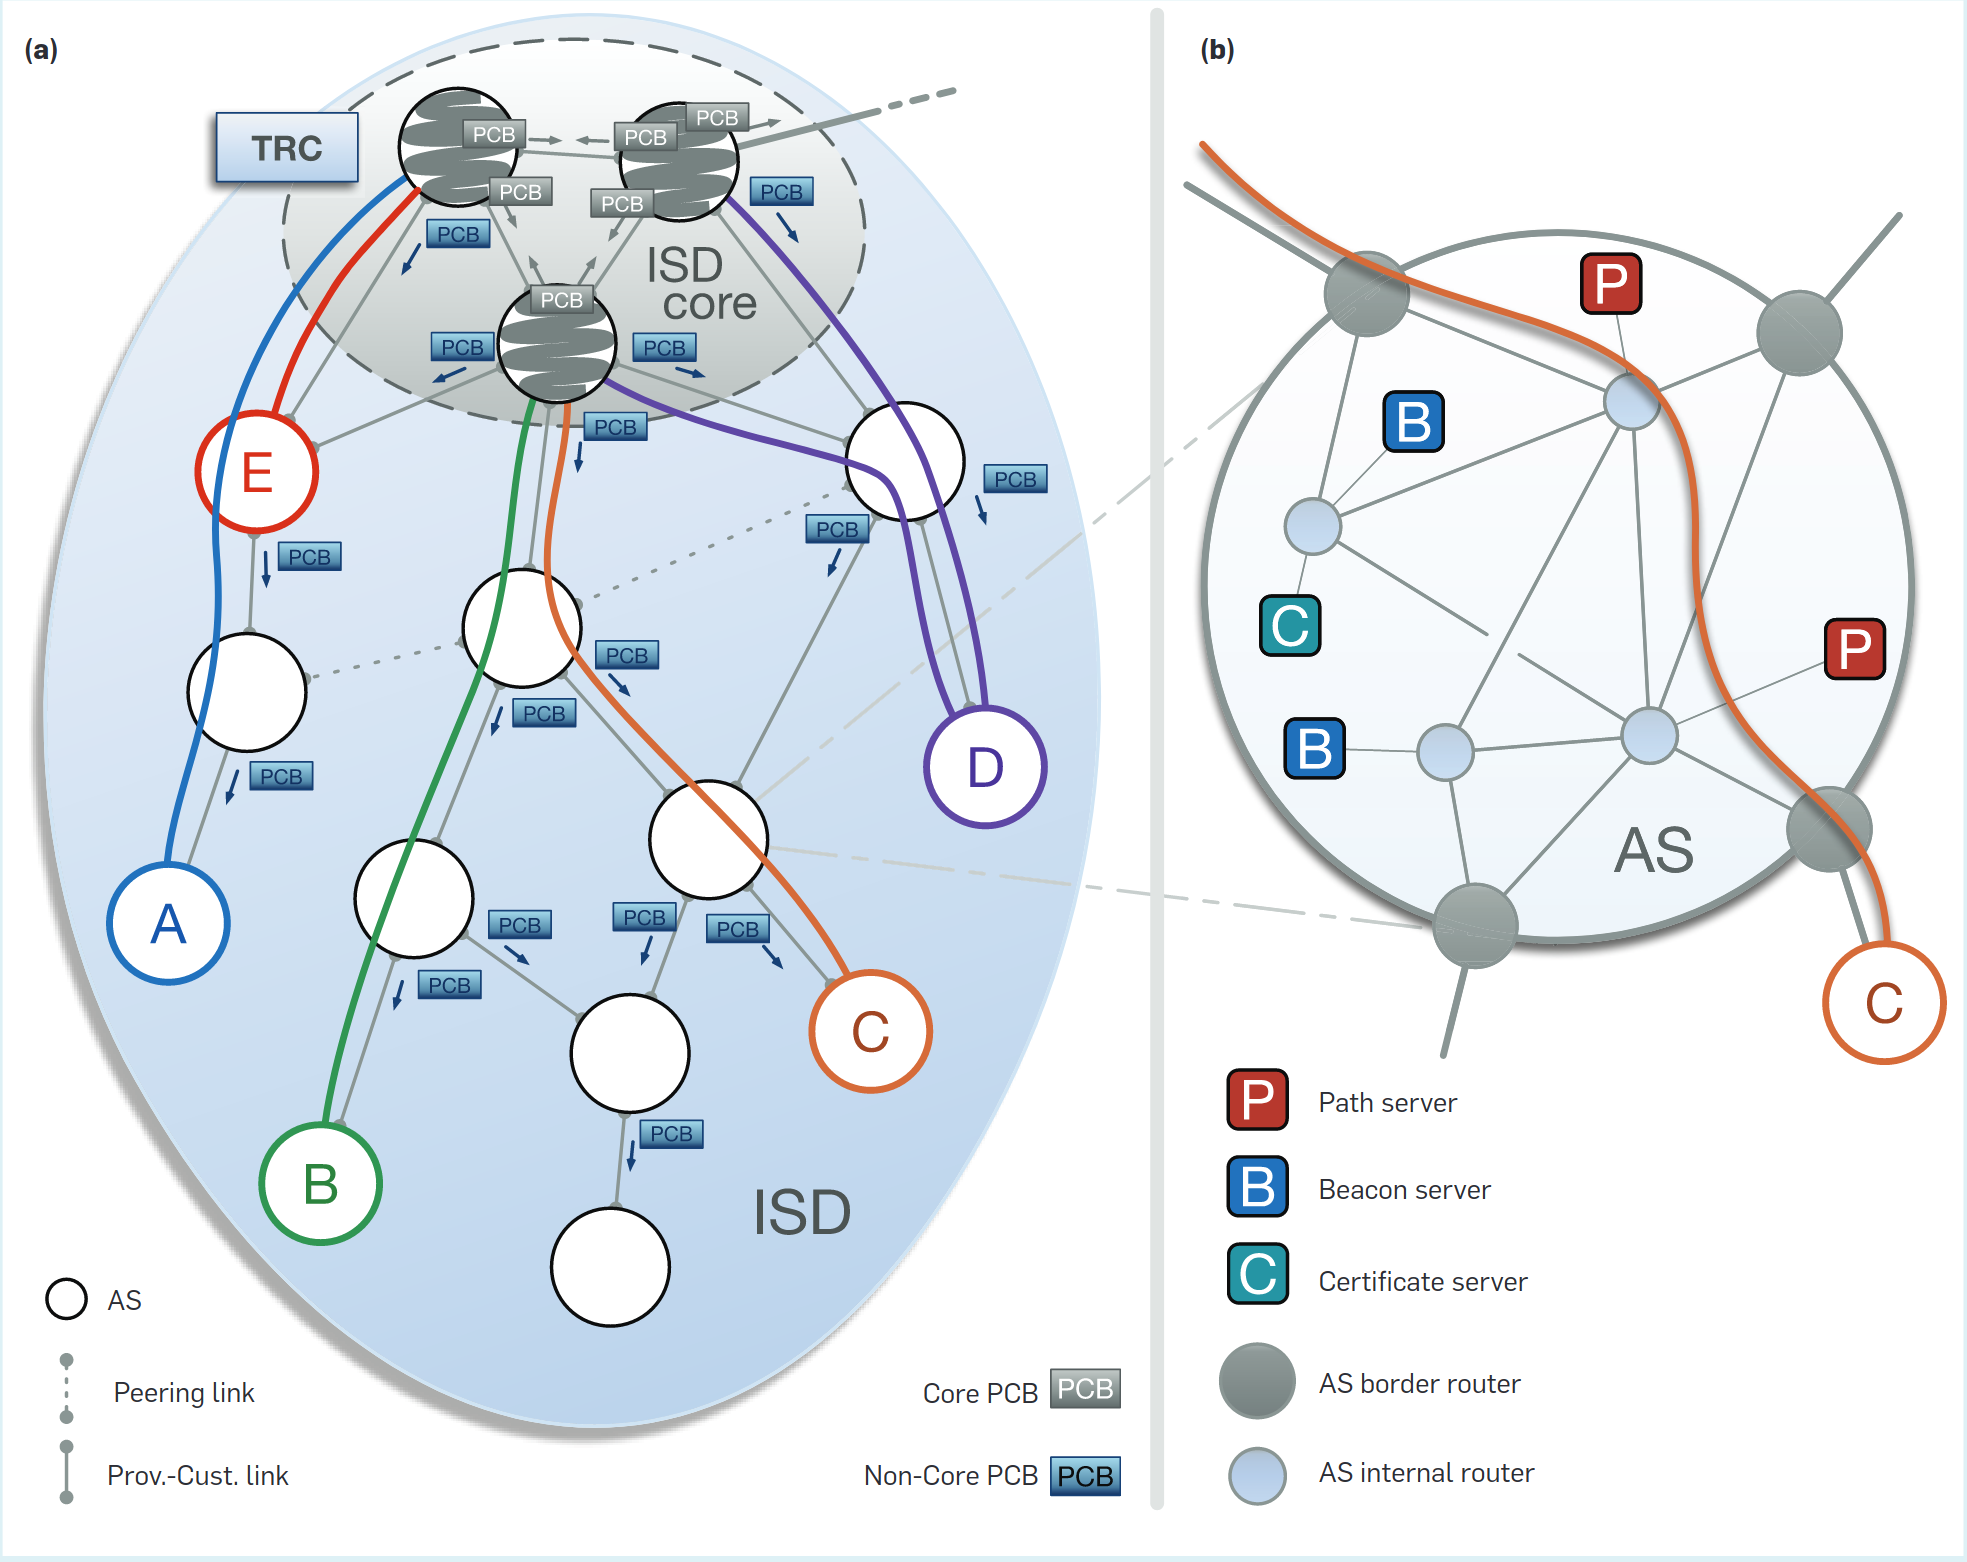
\includegraphics[width=0.8\linewidth]{scion_isd.png}
        \caption{Internal structure of an ISD. Image taken from \cite{scion_2015}}
        \label{fig:isd}
    \end{figure}

    PCBs travelling down collect what are called down-paths, but since all paths forward packets bidirectionally, each down-segment can be converted into an up-segment by inverting the order or traversed ASes. This one way propagation of PCBs has an important consequence: An AS always knows an up-path back to the ISD core, but it does not know how to reach other AS or ISDs, thus down-paths to other ASes must always be queried from the paths servers in the ISD core. Once an AS has received a number of path-segments, it can register some of them as down-paths segments with the core path servers in the ISD core. This gives an AS control over which down-paths are made available to other ASes, and creates the unique ability to control by which paths it wishes to be reached.

    When selecting down-paths, an AS tries to select as diverse paths as possible in order to reach maximum redundancy. This makes SCION an inherently multipathed system. Apart from path diversity, ASes can select for a number of different quality measure in their paths like low latency or anonymous forwarding capability along the whole path \cite{scion_2011}.

    So fare, we have looked at intra ISD path discovery. Inter ISD path discovery works much the same way; however, the PCBs are only forwarded between core ASes.

    \subsubsection{SCION Message Control Protocol} \label{sssec:scmp}
    The control plane comes with its own control protocol, the \textit{SCION Message Control Protocol} (SCMP). As its name already suggests, it operates quite similar to the already established ICMP protocol and serves many of the same functions \cite{scion_2015}. One noteworthy aspect of SCMP is that, in contrast to its cousin, it is integrity protect. For efficiency reasons, a MAC generated by a per-AS symmetric key is preferred over digital signatures. In the event a transit AS needs to send a SCMP message to a source AS, the per-AS key is generated on demand using the \textit{Dynamically Recreatable Keys} (DRK) algorithm and a common secret key shared among the ISDs border routers. The source AS (of the packet which caused the SCMP message) can then fetch the key from the transit AS sending the SCMP message, in case it does not already have it cached \cite{scion_2015}. 

    \subsection{Data Plane} \label{ssec:data_plane}
    While the control plane deals with path discovery, the data plane deals with forwarding data packets. For this task, the data plane uses the path information supplied by the control plane to assemble paths.

    \subsubsection{Packet Carried Forwarding State}\label{sssec:pcfs}
    In SCION, information needed to reach a forwarding decision for a given packet is stored in the packet itself. This is referred to as \textit{Package Carried Forwarding State} (PCFS) and several interesting properties of SCION are derived from this. Each packet at least contains a path, since source and destination addresses are optional, if the path is unambiguous in its context. Consequently, during forwarding, a router only needs to read the opaque field in the path and check its MAC in order to forward the packet to the next AS. Since all routing information is carried by the packet, the need for routing tables is eliminated.

    SCION splits the addressing information of a resource into a locator (the path) and an identifier (the destination address), which facilitates another interesting feature: Only the destination AS needs to be able to interpret the destination address. This allows each AS to choose its own addressing schema. As a consequence,   e.g., IPv4 and IPv6 hosts can talk directly to each other using SCION.

    The absence of routing tables simplifies the routings process and thus allows the construction of simpler and more energy-efficient machines. XY have observed a gain of xx  energy efficiency compared to traditional BGP routing. Thanks to hardware acceleration of cryptographic operations through technologies like Intel AES-NI, forwarding decisions in SCION become faster than in BGP. All a router needs to do is checking the validity of the path recorded in the packet and read the exit interface from it. If hardware acceleration is available, the signature validation is so efficient, it outperforms memory look-ups a BGP router needs to perform to reach its routing decision. 

    \subsubsection{Path Combination} \label{sssec:path_assembly}
    Path combination is the process performed by an end host to obtain a valid path before sending a packet. Up to three path-segments are combined into an end-to-end path. First, the end host looks up the AS and address of the destination with a name server. Then it queries a path server for a path to this destination. After the look-up process is complete, one of five scenarios will play out, depending on where the destination is located:

    \begin{itemize}
        \item \textbf{On path} (as shown in figure \ref{fig:isd}a $A \rightarrow E$) the destination lies directly on the up-path to the ISD core. The path is valid without any further processing. The up-path is truncated at the destination AS.
        \item \textbf{Direct combination} (as shown in figure \ref{fig:isd}a $B \rightarrow D$) The path can be constructed by chaining an up-segment with a down segment. The up- and down-segment intersect in a core AS.
        \item \textbf{AS shortcut} (as shown in figure \ref{fig:isd}a $B \rightarrow C$) This scenario is similar to the direct combination, but the destination lies on a down-segment which intersects the up-segment in a none core AS on the way to the ISD core. The unused segments up to the ISD core and back down to the intersection point are discarded.
        \item \textbf{Core path combination} (as shown in figure \ref{fig:isd}a $A \rightarrow D$) A up- and down-path do not intersect at any point and need to be connected by a core path-segment. This can either be an intra ISD or inter ISD path. This is one of three ways of traversing ISD borders.
        \item \textbf{Peering shortcut} (as shown in figure \ref{fig:isd}a $A \rightarrow B$) The up-segment and the down segment are connected by a peering link, such that the peering link allows a shortcut to the destination. Analogous to the AS shortcut, in this case the extraneous path segments are discarded as well. Note that this type of shortcut can also traverse ISD borders.
    \end{itemize}

    Once the host has constructed a path, it is encoded as PCFS in the packet header. The destination host can either take the path contained it the received packet and simply reverse it, or perform its own lookup and combination process. Of course, this process is assisted by various cashing mechanisms.

    \subsubsection{Source Routing and Path Transparency} \label{sssec:source_routing}
    One of SCION's biggest claims to fame is its secure and efficient implementation of source routing. Source routing means that the source of a data packet determines the route the packet will travel along to its destination. The path construction process described in the previous section is performed on the end host sending a data packet providing exactly this source routing feature. The path information is stored as PCFS data (see section \ref{sssec:pcfs}) in the packet header and is cryptographically protected against tampering. This not only guarantees that the packet will be routed on the selected path, but also creates path transparency for the destination end host.

    \subsection{Isolation of Attacks}
    SCION carves the global internet up into smaller self-contained units through ISDs, and even these can be subdivided  into  subISDs. This by itself already provides a significant advantage, since all entities outside an ISD cannot influence the path discovery process (see section \ref{sssec:beaconing}). Further, the compromise of a trust roots is isolated to an ISD as well and may not affect other ASes in other ISDs.

    Attacks are further isolated in that no AS can influence the path construction process (see section \ref{sssec:path_assembly}) taking place on an end host. A malicious AS can only announce down-paths to reach that malicious AS. PCFS information is MAC protected, the chosen path for a packet cannot be altered by a malicious AS on the path. 

    \subsection{Trust Management and Trust Agility}
    As stated in the introduction, trust management is a hard problem to solve, and SCION takes a few important steps towards solving this problem. First of all the architecture limits the scope of trust to a smaller set of trustees by introducing ISDs, secondly it reduces the number of trust roots to a manageable number \cite{scion_2011}. This makes key revocation, or certificate revocation respectively, much more feasible.  There is no need for every single end host on the entire Internet to be informed individually. SCION also makes extensive use of trust transitivity offered by digital signatures.

    Trust agility is the concept that the user can choose which roots of trust they relay upon and that they can revoke their trust, quickly and effectively, if an entity is compromised. This requires a simple and quick key revocation process, which SCION aims to provide this by effectively avoiding two scenarios:

    \begin{itemize}
        \item \textbf{Trust monopoly}: All the entities on the internet need to trust one root of trust, like in DNSSEC or BGP Sec. This scenario suffers from having a single point of failure, and revoking a key in this system is going to create an administrative nightmare that affects the whole infrastructure.
        \item  \textbf{Trust oligopoly}: In this scenario, there is a multitude of equally trusted roots of trust. An example for this is the current  TLS PKI system. This scenario suffers from the fact that it exposes many points of failure, and that each trust root can sign certificates for arbitrary entities. Revoking keys is made difficult by the sheer number of keys to manage. This trust model is only as strong as its weakest link.
    \end{itemize}

    This is achieved by introducing a hierarchy of trust. \cite{scion_2011}. ASes use several different keys for different purposes and can replace the keys and employed algorithms autonomously. However, the used keys always require a signature by a trust root. This enables neighbouring ASes and end host in different ASes or ISDs to check the validity of the keys and by extensions the data processed by these keys. The keys used for this signing are encoded in the TRC and are thus managed and protected by the ISD core.

    In SCION, trust is rooted in a low number of trust roots, which are encoded in each ISDs TRC. This TRC is only valid inside the ISD it applies to, thus limiting the scope of trust to one ISD. Since linked ISDs signed each other's TRCs trust is conveyed, by the transitive properties of trust, between ISDs. If an ISD revokes a trust root's key, all keys signed with it, become invalid at once. This change propagates quickly through the ISD own ASes as well as to neighbouring ISDs by the means of PCBs. From this, an interesting property emerges: As long as there is a path available to a given resource, the path can always be validated.

    \section{SCION Extensions}
    When SCION was first conceptualized, the idea was to incorporate all needed features in a holistic design. However, the authors acknowledged the need for SCION to be extensible, since not all features are vital to SCIONS proper operation. We will have a brief look at some of the more noticeable ones here.

    Through source routing, SCION already allows an end host to route around ASes it does not trust \cite{scion_2011}; however, this is insufficient protection if a sender wants to remain truly anonymous. Therefore, XY et al. propose the \textit{High-speed Onion Routing at the Network-Level} \cite{hornet_2015, hornet_2016} or HORNET extension, which aims to add onion routing \cite{onion_routing} to the protocol. The opaque fields and PCFS feature of SCION make it uniquely suited to onion routing, since an AS only needs to be able to read the opaque field it itself has created and does not depend on any knowledge about the preceding and following ASes in the path.

    The SCION protocol already offers defences against DDoS attacks by giving ASes the ability to keep some down paths hidden until they are needed in an emergency \cite{scion_2015}. To further harden SCION against DDoS attacks, Basescu et al. propose the \textit{Scalable Internet Bandwidth Reservation Architecture} \cite{sibra_2016} or SIBRA extensions. The extension introduces defences against link-flooding attacks such as Coremalt \cite{coremelt} and Crossfire \cite{crossfire} attacks, which aim to degrade the performance of backbone links or the target itself by overwhelming them with what looks like legitimate traffic. SIBRA combats DDoS attacks by a combination of contractual agreements for bandwidth reservation and technical measures to enforce these reservations \cite{sibra_2016}.

    SCION is designed with easy adoption in mind and offers a number of attractive benefits to adopters. Design elements such as the use of existing ASes and isolating the inner structure of an AS from the SCION architecture are specifically targeted at easy adoption of SCION. For an AS to adopt SCION, it only needs to deploy border routes which are SCION capable, as well as deploying name, beacon, certificate, and path servers. All these can run on commodity hardware, while the rest of the AS can remain largely unchanged. Since core elements from BGP are adopted like ASes and beaconing, BGP routing policies can be fully expressed and even extended in SCION, further lowering the bar of entry to adopting SCION \cite{scion_2017}.

    Since 2016 a real-world SCION test bed called ScionLab is operational \cite{testbed_2020} which includes several high-profile members such as Swisscom and Switch, as well as other financial institutions like SIX and the Swiss National Bank \cite{snb} and further academic institutions. In fact, as of 2020, the test bed serves over 600 entities and spans a global network around 40 ISDs.

\end{document}
